\documentclass[11pt]{article}

\usepackage[letterpaper,margin=0.75in]{geometry}
\usepackage{booktabs}
\usepackage{graphicx}
\usepackage{listings}
\usepackage{hyperref}

\setlength{\parindent}{1.4em}

\begin{document}

\lstset{
  language=Python,
  basicstyle=\small,          % print whole listing small
  keywordstyle=\bfseries,
  identifierstyle=,           % nothing happens
  commentstyle=,              % white comments
  stringstyle=\ttfamily,      % typewriter type for strings
  showstringspaces=false,     % no special string spaces
  numbers=left,
  numberstyle=\tiny,
  numbersep=5pt,
  frame=tb,
}

\newenvironment{absolutelynopagebreak}
  {\par\nobreak\vfil\penalty0\vfilneg
   \vtop\bgroup}
  {\par\xdef\tpd{\the\prevdepth}\egroup
   \prevdepth=\tpd}

\title{Network Simulation}

\author{Cody Heffner}

\date{7 Mar. 2015}

\maketitle

\section{Preface}

This report details the experiment I ran and the results obtained as specified by the Congestion Control Lab in the BYU CS 460 class taught by Dr. Zappala. The project specifications can be found \href{http://cs460.byu.edu/winter-2015/labs/congestion-control-part-1}{here}.

The experiment requires heavy use of a network simulator to test different network scenarios. The network simulator I used is Dr. Zappala's \href{https://github.com/zappala/bene}{Bene}, written in Python. All my simulation examples shown will be tailored towards use for that simulator.

\section{Summary}

The goal of this lab was to implement TCP congestion control in my implementation of TCP. This includes implementing TCP slow start and TCP additive increase, multiplicative decrease, as well as a fast-retransmit function.

\section{Congestion Control}

Congestion control in TCP is achieved by restricting the maximum number of segments TCP is able to send at one time. TCP starts by sending only a few segments of data at a time and waiting until the receiver sends an acknowledgement (ACK) back to the sender. Each time an ACK is received by the sender, the sender increases the maximum number of segments it is able to send. When the sender is in slow start mode, this maximum number of segments it is able to send is doubled each time a set of ACKs are received. When the sender is in additive increase mode, the maximum number of segments it is able to send is increased by one each time a set of ACKs are received.

When no ACKs are received before a timer expires, or if the sender receives duplicate events, this indicates a loss event. The sender handles a loss event by halving the threshold of maximum segments it is allowed to send and resetting to one the current number of segments it is sending.

I implemented congestion control with just a couple of functions. I created a lossevent function that resets the threshold and the current window, and an increasewindow function that checks for duplicate ACKs, then calling the lossevent function or increasing the window based on whether it should be in additive increase or slow start. The following code shows these functions.

\vspace{5mm}
\begin{absolutelynopagebreak}
\begin{lstlisting}
def loss_event(self):
    self.threshold = max(self.window/2, self.mss)
    self.window = 1 * self.mss

# slow start & AI
def increase_window(self, amount):
    # loss event check
    self.duplicates += 1
    if amount == 0 and self.duplicates >= 4:
        self.loss_event()
    else:
        self.duplicates = 0

        # AI
        if amount + self.window >= self.threshold:
            self.window += (self.mss * amount / self.window)
            self.threshold = self.window
        # slow start
        else:
            self.window += amount
\end{lstlisting}
\end{absolutelynopagebreak}
\vspace{5mm}

\section{Tests}

Slow Start: To test slow start, I transferred a small file that transferred entirely within the range of slow start. In the following graph, the reader should notice that each set of segments doubles in size. 

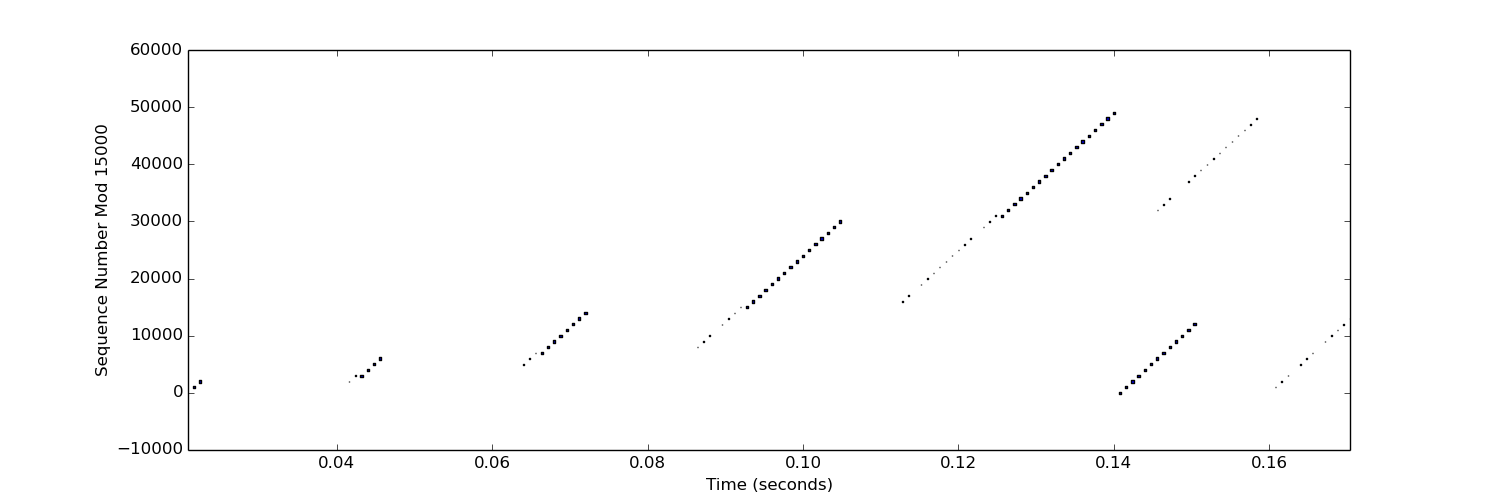
\includegraphics[width=17cm]{outputs/converted_output1.png}

Additive Increase: To test additive increase, I transferred a larger file with a threshold of 16,000 bytes, i.e., 16 segments.  The reader can observe in the following graph that each set of segments doubles in size, like in the previous graph, until the sender sends 16 segments. The next set is 17 segments in size, and the final set is also 17 segments in size, which concluded the file transfer.

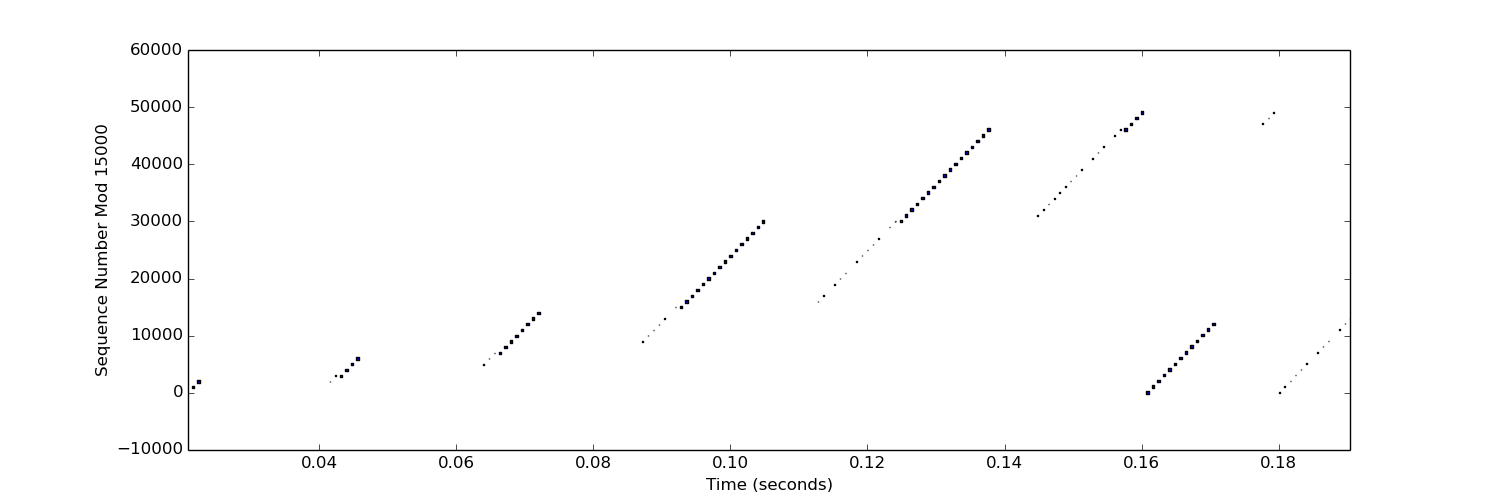
\includegraphics[width=17cm]{outputs/converted_output2.png}

\end{document}
